\Level 0 {Basic terminology}

Terminology of fonts and typefaces is quite confused these
days. Traditionally, a \index{typeface}typeface was a design, realized
in number of fonts, that could be sorted in families, such as roman,
and italic. A~\index{font}font would then be a style (medium weight
bold italic) in a particular size. 

Somewhat surprisingly, once you start throwing computers at this
problem, even talking about characters becomes very subtle.

In Unicode, there are abstract characters and characters. They don't
differ by much: an abstract character is a concept such as `Latin
lowercase a with accent grave', and a character is that concept plus a
position in the Unicode table. The actually visible representation of
a character is called a `\index{glyph}glyph'. According to
\index{ISO!9541}ISO~9541, a glyph is `A~recognizable abstract graphic
symbol which is independent of any specific design'.

\Level 1 {The difference between glyphs and characters}

Often, the mapping between character and glyph is clear: we all know
what we mean by `Uppercase Roman~A'. However, there may be 
\begin{figure}
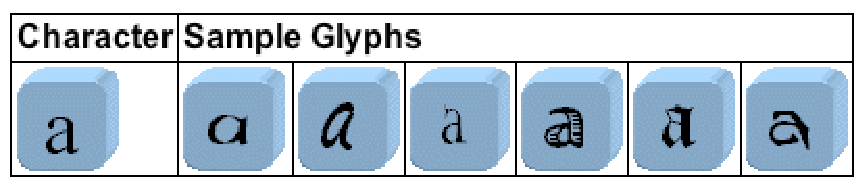
\includegraphics[scale=.7]{a-glyphs}
\caption{Different shapes of `lowercase roman~a'}\label{fig:a-glyphs}
\end{figure}
different glyph shapes that correspond to the same character.

An abstract character is defined as
\begin{quotation}
abstract character: a unit of information used for the organization,
control, or representation of textual data.
\end{quotation}
This definition has some interesting consequences. Sometimes one glyph
can correspond to more than one character, and the other way around.

For example, in Danish, the ligature `\ae' is an actual character. On
the other hand, the
ligature~`fl', which appears in English texts, is merely a
\begin{figure}[ht]
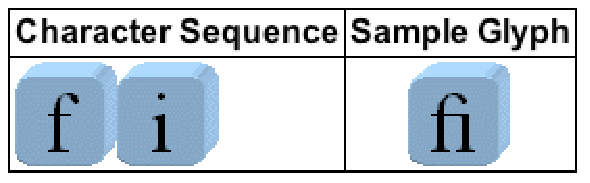
\includegraphics[scale=.7]{fi-ligature}
\caption{The f-i ligature}\label{fig:fi-ligature}
\end{figure}
typographical device to make the combination `f{}l' look better, so
one glyph corresponds to two characters.

The opposite case is rarer. In Tamil, a~certain character is split,
\begin{figure}
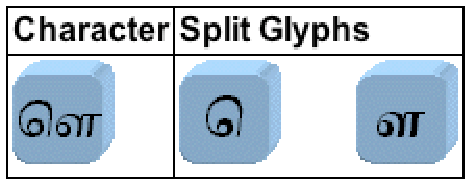
\includegraphics[scale=.7]{Tamil-split}
\caption{A split character in Tamil}\label{fig:tamil-split}
\end{figure}
because it is positioned \emph{around} other characters. It can then
even happen that one of the split parts forms a ligature with adjacent
characters.

A~tricker question is how to handle accented letters: is `\'e' one
character or a combination of two? In math, is the relation in
\begin{figure}[ht]
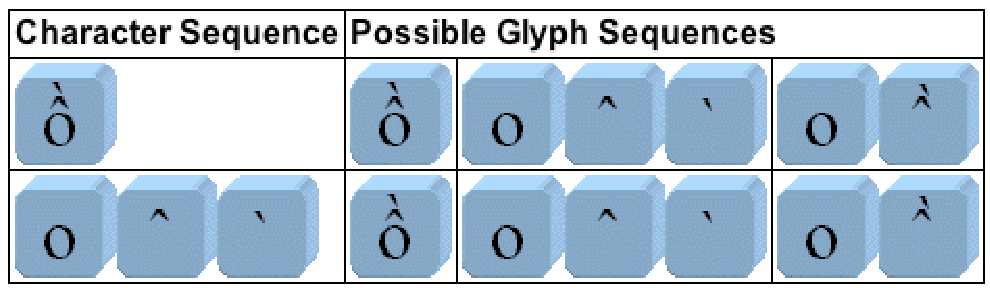
\includegraphics[scale=.7]{o-accents}
\caption{Different interpretations of an accented character glyph}
\label{fig:o-accent}
\end{figure}
$a\not=b$ {\em one} symbol, or an overstrike of one over another?

Another problem with ligatures is that a single glyph needs to be
displayed, but two glyphs need to be stored to make searching for the
string possible.

\Level 1 {The identity of a character}

Another problem in defining a character is whether two glyphs that
look the same, or sometimes ever {\em are} the same, should be the
same character. For example, uppercase Latin~a, uppercase
Greek~$\alpha$, and uppercase Cyrillic~a, are all rendered~`A'. Still,
in Unicode they are three distinct characters.

Similarly, in \ascii, there are no separate glyphs for minus, hyphen,
and dash. In Unicode, these are three characters. Is the character
`superscript~$^2$' a separate glyph, or a typographical variant of the
character `digit~2'? The latter should be the logical solution, but
for compatibility reasons with other standards it is defined as a
separate glyph. There are quite a few of these `\index{compatibility
  characters (Unicode)}compatibility characters.

Yet another example is the Greek letter~$\Omega$, which can be that
letter, or the sign for electrical resistance in physics
texts. Unicode defines them as two characters, but with identical
glyphs.

A~capital `A' in Times Roman and in Helvetica are the same character,
but what about italic?

All these matters are hard to settle objectively: everything is a
matter of definition, or a judgement call. The official Unicode white
paper on characters versus glyphs is
\url{http://www.unicode.org/reports/tr17/}.

Here are some of the guidelines of the Unicode project:
\begin{itemize}
\item The Unicode Standard encodes characters, not glyphs.
\item Characters have well-defined semantics.
\item The Unicode Standard encodes plain text.
\item And:
\begin{quotation}
The Unicode Standard avoids duplicate encoding of characters by
unifying them within scripts across languages; characters that are
equivalent in form are given a single code. Common letters,
punctuation marks, symbols, and diacritics are given one code each,
regardless of language, [\dots]
\end{quotation}
\end{itemize}

\Level 1 {Diacritics}

Unicode, a bit like \TeX, has two ways of dealing with diacritics. It
has precomposed accented characters, but it can also compose accented
characters by listing accents (yes, plural: transliterated Vietnamese
regularly has two accents over a letter one relating to vowel quality,
and one to tone) after the base symbol. This
mechanism can also deal with languages such as Hangul (Korean) which
have composite characters.

\Level 0 {\AE sthetics}

\Level 1 {Scaling versus Design sizes}
\label{sec:design-size}

Lots of attention is devoted to font scaling, with the implicit assumption that
that is the way to get a font to display at different sizes. This is
only true to an extent: a small version of a typeface was
traditionally of a different design than the same typeface at larger
sizes. With metal type, independent designs for the different sizes
were of course the only way one could proceed at all, but with photo
typesetters and computers the need went away, and with it the
realization that independent designs are visually actually a Good
Thing.
\begin{figure}[ht]
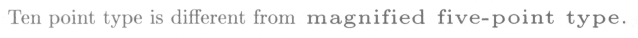
\includegraphics{design-size}
\caption{A typeface and a smaller version scaled up}
\label{fig:design-size}
\end{figure}
Figure~\ref{fig:design-size} shows the difference between a typeface
set at its `\index{design size}design size', and a scaled up smaller
version of it.

\begin{figure}[ht]
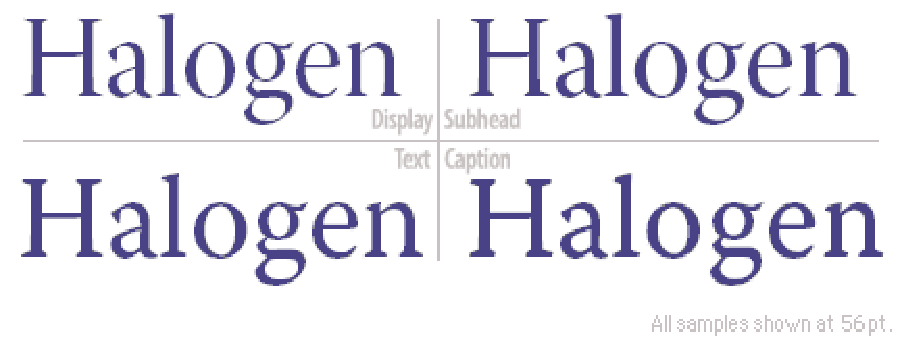
\includegraphics[scale=.6]{optical-masters}
\caption{Adobe's optical masters for a typeface}
\label{fig:optical-master}
\end{figure}
Adobe incorporated this idea in their \index{Multiple Master font
  technology}Multiple Masters typefaces, which could interpolate
between different designs. This technology seems to have been
abandoned, but Adobe's Originals now have so-called `\index{Optical
  masters}Optical masters: four different designs of the same
typeface, to be set at different sizes. Adobe labels their purposes as
`display', `subhead', `text', and `caption' in decreasing design size;
see figure~\ref{fig:optical-master}.

Apple developed their own version of multiple design sizes in TrueType
GX, released in 1994. The ideas in TrueType GX are incorporated in
Apple Advanced Typography (AAT) in OS~X, but there few AAT typefaces,
and certainly very few non-Apple ones.

\Level 0 {Font technologies}

\Level 1 {Unicode in fonts}
\label{sec:unicode-font}

It is unrealistic to expect any single font to support even a decent
fraction of the Unicode character repertoire. However, TrueType and
OpenType do support Unicode.

The few fonts that support (almost) the whole of Unicode are called
`pan-Unicode'. There are only a few of those. However, software these
days is pretty sophisticated in gathering together symbols from
disparate fonts. Some browsers do this, prompting the user for
`install on demand' of fonts if necessary.

\Level 1 {Type 1 and TrueType}

% material stolen from
% \url{http://www.truetype.demon.co.uk/articles/ttvst1.htm}

\index{Font!Type 1}Type~1 (`\index{Font!Postscript}Postscript fonts')
was the outline font format developed by Adobe that was adopted by
Apple in the mid 1980s. Since it was proprietary (Adobe had release
the specifications for \index{Font!Type 3}Type~3 fonts, but not
Type~1), Apple and Microsoft later developed
\index{Font!TrueType}TrueType.

With Type~1 fonts, information is stored in two files, one for shape
data and one for hinting and such. With TrueType, all information is
in the one font file.

\Level 2 {Type1}

% this section stolen
% from \url{http://www.math.utah.edu/~beebe/fonts/postscript-type-1-fonts.html}

Adobe Type 1 fonts are stored in two common formats, .pfa (PostScript
Font ASCII) and .pfb (PostScript Font Binary). These contain
descriptions of the character shapes, with each character being
generated by a small program that calls on other small programs to
compute common parts of the characters in the font. In both cases, the
character descriptions are encrypted.

Before such a font can be used, it must be rendered into dots in a
bitmap, either by the PostScript interpreter, or by a specialized
rendering engine, such as Adobe Type Manager, which is used to
generate low-resolution screen fonts on Apple Macintosh and on
Microsoft Windows systems.

The Type 1 outline files do not contain sufficient information for
typesetting with the font, because they have only limited metric data,
and nothing about kerning (position adjustments of particular adjacent
characters) or ligatures (replacement of adjacent characters by a
single character glyph, those for fi, ffi, fl, and ffl being most
common in English typography).

This missing information is supplied in additional files, called .afm
(Adobe Font Metric) files. These are ASCII files with a well-defined
easy-to-parse structure.  Some font vendors, such as Adobe, allow them
to be freely distributed; others, such as Bitstream, consider them to
be restricted by a font license which must be purchased.

\Level 2 {TrueType $\Leftrightarrow$ Type1 conversion}

Beware! There is no such thing as a one-to-one reversible
conversion. There are several problems:

The outlines are stored in different ways in both formats. In
truetype, second-order Bezier curves are used, and in type 1,
third-order Bezier curves are employed. One second order Bezier can be
transformed into a third-order Bezier, but a third-order Bezier cannot
be transformed into one, two or seventeen second-order
Beziers--approximations are in order for that conversion. So, type 1
to truetype is problematic, right from the start. For truetype to type
1, there is a snake in the grass, in the form of integer grid rounding
(see below).


Both formats require all control points to be integers (whole
numbers), falling in a grid. Truetype uses a 2048x2048 grid, type 1
typically a 1000x1000 grid. For the truetype to type 1 direction, one
could divide all grid values by two, but then what? Should 183.5
become 183 or 184? The type 1 to truetype direction is easier, at
least from this point of view, as we could multiply each grid
coordinate by two, so no rounding loss would be involved. However, in
the truetype to type 1 direction, the rounding causes additional
problems for the new control points needed for the perfect third-order
Bezier outlines mentioned above.


Placing ink on paper: the formats have different rules for placing ink
on paper in case of outlines that are nested or intersecting. These
differences are not caught by many conversion programs. In most cases,
the user should not worry about this---only rarely do we have
overlapping outlines (I was forced once to have them, for other
reasons).


Complexity of the outlines: truetype permits more complex outlines,
with more control points. For example, I am sure you have all seen
fonts made from scans of pictures of faces of people. Typically, these
outlines are beyond the type 1 limit, so this restriction makes the
truetype to type 1 conversion impossible for ultra complex fonts.

Encoding: truetype can work with a huge number of glyphs. There are
truetype fonts for Chinese and Japanese, for example. In type 1, the
number of active glyphs is limited to 256. Again, for most Latin
fonts, this is a non-issue.

The remarks about grid rounding also apply to all metrics, the
bounding boxes, the character widths, the character spacing, the
kerning, and so forth.

Finally, there is the hinting. This is handled very differently in
both formats, with truetype being more sophisticated this time. So, in
truetype to type 1 conversions of professionally (hand-hinted) fonts,
a loss will occur. Luckily, 99\% of the truetype fonts do not make use
of the fancy hinting possibilities of truetype, and so, one is often
safe.

All this to tell people to steer away like the plague from format
conversions. And a plea to the font software community to develop one
final format. My recommendation: get rid of truetype, tinker with the
type 1 format (well, tinker a lot). More about that ideal format
elsewhere.

\Level 2 {Downsampling bitmaps}

In principle, given adequate resolution, the screen preview quality of
documents set in bitmap fonts, and set in outline fonts, should be
comparable, since the outline fonts have to be rasterized dynamically
anyway for use on a printer or a display screen.

Sadly, this is not the case with versions of Adobe Acrobat Reader,
acroread, and Exchange, acroexch (version 5.x or earlier); they do a
poor job of downsampling high-resolution bitmap fonts to
low-resolution screen fonts. This is particularly inexcusable,
inasmuch as the co-founder, and CEO, of Adobe Systems, is the author
of one of the earliest publications on the use of gray levels for font
display: [ John E. Warnock, The display of characters using gray level
sample arrays, Computer Graphics, 14 (3), 302--307, July, 1980.  ]

\Level 1 {FreeType}

\index{FreeType}FreeType is an Open Source implementation of
TrueType. Unfortunately this runs into patent problems, since Apple
has patented some of the hinting mechanism. Recently FreeType has
acquired an automatic hinting engine.

\Level 1 {OpenType}

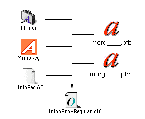
\includegraphics{opentype}
\index{OpenType}OpenType is a standard developed by Adobe and
Microsoft. It combines bitmap, outline, and metric information in a
single cross-platform file. It has Unicode support, and can use
`Optical Masters' (section~\ref{sec:design-size}) multiple designs. It
knows about the distinction between code points and glyphs, so
applications can render a character differently based on context.

\Level 0 {Font handling in \TeX\ and \LaTeX}

\TeX\ has fairly sophisticated font handling, in the sense that it
knows a lot about the characters in a font. However, its handling of
typefaces and relations between fonts is primitive. \LaTeX\ has a good
mechanism for that.

\Level 1 {\TeX\ font handling}

Font outlines can be
stored in any number of ways; \TeX\ is only concerned with the
`\index{font metrics}font metrics', which are stored in a `\index{tfm
  file}\n{tfm} file'. These files contain
\begin{itemize}
\item Global information about the font: the \cs{fontdimen}
  parameters, which describe the spacing of the font, but also the
  x-height, and the slant-per-point, which describes the angle of
  italic and slanted fonts.
\item Dimensions and italic corrections of the characters.
\item Ligature and kerning programs.
\end{itemize}
We will look at these in slightly more detail.

\Level 2 {Font dimensions}

The \n{tfm} file specifies the natural amount of space, with stretch
and shrink for a font, but also a few properties related to the size
and shape of letters. For instance, it contains the x-height, which is
the height of characters without ascenders and descenders. This is,
for instance,
used for \index{accents}accents: \TeX\ assumes that accents are at the
right height for characters as high as an~`x': for any others the
accent is raised or lowered.

The `slant per point' parameters is also for use in accents: it
determines the horizontal offset of a character.

\Level 2 {Character dimensions}

The height, width, and depth of a character is used to determine the
size of the enclosing boxes of words. A non-trivial character
dimension is the `\index{italic correction}italic correction'. A~tall
italic character will protrude from its bounding box (which apparently
does not always bound). The italic correction can be added to a
subsequent space.
\begin{quote}
`\TeX\ has' versus `\TeX\/ has'
\end{quote}

\Level 2 {Ligatures and kerning}

The \n{tfm} file contains information that certain sequences of
characters can be replaced by another character. The intended use of
this is to replace sequences such as \n{fi} or \n{fl} by `fi' or~`fl'.

Kerning is the horizontal spacing that can bring characters closer in
certain combinations. Compare
\begin{quote}`Von' versus `\hbox{V}\hbox{on}'
\end{quote}
Kerning programs are in the \n{tfm} file, not accessible to the user.

\Level 1 {Font selection in \LaTeX}

Font selection in \LaTeX\ (and \TeX) was
rather crude in the early versions. Commands such as \cs{bf} and
\cs{it} switched to boldface and italic respectively, but could not be
combined to give bold italic. The \index{NFSS}New Font Selection
Scheme improved that situation considerably.

With NFSS, it becomes possible to make orthogonal combinations of the
font family (roman, sans serif), series (medium, bold), and shape
(upright, italic, small caps).
A~quick switch back to the main document font is \cstoidx{textnormal}
or \cstoidx{normalfont}.

\Level 2 {Font families}

It is not necessary for a typeface to have both serifed and serifless (sans
serif) shapes. Often, therefore, these shapes are taken from different, but
visually compatible typefaces, for instance combining Times New Roman
with Helvetica. This is the combination that results from
\begin{verbatim}
\usepackage{times}
\end{verbatim}
Loading the package \n{lucidabr} instead, gives Lucida Bright and
Lucida Sans.

The available font families are
\begin{description}
\item[roman] using the command \cstoidx{textrm} and the declaration
  \cstoidx{rmfamily}.
\item[sans serif]  using the command \cstoidx{textsf} and the declaration
  \cstoidx{sffamily}.
\item[typewriter type] using the command \cstoidx{texttt} and the
  declaration \cstoidx{ttfamily}. Typewriter type is usually a
  monospaced font -- all characters of the same width -- and is useful
  for writing about \LaTeX\ or for giving code samples.
\end{description}

\Level 2 {Font series: width and weight}

The difference between normal and medium width, or normal and bold
weight, can be indicated with font series commands:
\begin{description}
\item[medium width/weight] using the command \cstoidx{textmd} and the
  declaration \cstoidx{mdseries}.
\item[bold]  using the command \cstoidx{textbf} and the declaration
  \cstoidx{bfseries}.
\end{description}

\Level 2 {Font shape}

The final parameter with which to classify fonts is their shape.
\begin{description}
\item[upright] This is the default shape, explicitly available through
  \cstoidx{textup} or \cstoidx{upshape}.
\item[italic and slanted] These are often the same; they are available
  through \cstoidx{textit}, \cstoidx{textsl}, and \cstoidx{itshape},
  \cstoidx{slshape}.
\item[small caps] Here text is set through large and small capital
  letters; this shape is available through \cstoidx{textsc} and
  \cstoidx{scshape}.
\end{description}

